\section{Newton's Laws of Motion}

%First Law / Inertia

%\subsection{Magic Card Trick}
%\begin{itemize}
%\item{Preparation Time: none}
%\item{Materials: empty soda bottle, card, heavy coin}
%\item{Procedure: Place the card over the mouth of the bottle and let the coin rest on top. Invite students to try to remove the card without moving the coin. Most will not be able to do it. Flick the card quickly from the side; it should fly off the bottle, leaving the coin resting neatly on top of the bottle.}
%\item{Theory: The coin has inertia, meaning it will resist any changes to its motion. Despite the friction from the card pulling the coin off the bottle, the coin will remain in place. This is also a good demonstration of impulse.}
%\end{itemize}


\subsection{Verification of Newton's First Law of Motion}

\subsubsection*{Learning Objectives}
\begin{itemize}
\item{To explain the concept of inertia} 
\item{To Verify Newton's first law of motion} 
\end{itemize}

\subsubsection*{Background Information}
An object will tend to resist changes to its motion. This is called inertia and is explained by Newton's first law of motion. This law states that ``an object at rest will tend to stay at rest unless acted upon by an external force. An object in motion well continue in that motion unless acted upon by an external force."  In short, this means that an object will continue doing what it is doing. The concept of inertia explains the reason why passengers move forward when the driver applies breaks, or fall back when the car starts moving suddenly.

\subsubsection*{Materials}
Empty soda bottle, small manila sheet OR card, knife, coin

\subsubsection*{Preparation Procedure}
Cut a small piece of card from the manila sheet.

\subsubsection*{Activity Procedure}
\begin{enumerate}
\item{Place the bottle on top of the table.} 
\item{Cover the mouth of the bottle with the card.} 
\item{Put a coin on top of the card on the rim of the bottle.} 
\item{Flick or quickly pull the piece of manila sheet horizontally off of the bottle.} 
\end{enumerate}

\begin{figure}
\begin{center}
%\def\svgwidth{200pt}
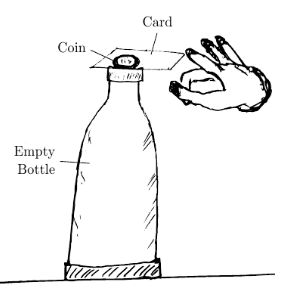
\includegraphics{./img/inertia.png}
\caption{Demonstration of Newton's First Law}
\label{fig:inertia}
\end{center}
\end{figure}

\subsubsection*{Results and Conclusions}
As you flick the piece of card quickly the card flies away and the coin remains in the same position (on top of the bottle rim). The coin remains at the same point due to its tendency to maintain its position. This property of resisting change to motion is called inertia.

\subsubsection*{Clean Up Procedure}
Return the materials to their proper places.

\subsubsection*{Discussion Questions}
\begin{enumerate}
\item{Discuss your daily experience with the concept of inertia.} 
\item{Design another way to demonstrate the concept of inertia.} 
\item{Explain why Newton's first law is known as the ``Law of Inertia."}
\end{enumerate}


%\subsection{Spinning Eggs}
%\begin{itemize}
%\item{Preparation time: none}
%\item{Materials: 2 eggs (1 boiled, 1 fresh)}
%\item{Procedure: Spin the eggs on their sides. If you briefly stop the fresh egg, then release it, it will begin to spin again by itself. However, if you briefly stop the boiled egg, it will remain stopped.}
%\item{Theory: The boiled egg is a rigid body, so when you stop its shell, you stop the whole egg. The fresh egg is not a rigid body. It has liquid inside, so when you stop the shell, the inside continues spinning. When you release it, the inside has enough angular momentum to start the whole thing spinning again.}
%\end{itemize}


\subsection{Inertia and Newton's First Law of Motion}

\subsubsection*{Learning Objectives}
\begin{itemize}
\item{To understand the concept of inertia} 
\item{To demonstrate Newton's First Law (the Law of Inertia)} 
\end{itemize}

\subsubsection*{Background Information}
Newton's first law, also called the Law of Inertia, states that "an object in motion will continue in that motion, and an object at rest will remain at rest unless acted upon by an external force". This simply means that an object will continue doing what it is doing and will resist any changes.  
The inside of a fresh egg is liquid while the inside of a boiled egg is solid. Therefore, if you change the motion of the shell of a fresh egg, the liquid inside will resist the change and continue with whatever motion it had. If you change the motion of a boiled egg shell, the inside of the egg will follow the same motion as the shell.  

\subsubsection*{Materials}
1 fresh egg and 1 boiled egg

\subsubsection*{Activity Procedure}
\begin{enumerate}
\item{Place both eggs on the table and note that it is impossible to tell which egg is fresh and which egg is boiled.} 
\item{Spin the first egg.} 
\item{While the egg is spinning, stop it briefly with your hand and then release the egg.  Record any observations.} 
\item{Spin the second egg.} 
\item{While the egg is spinning, stop it briefly with your hand and then release the egg.  Record any observations.} 
\end{enumerate}

\subsubsection*{Results and Conclusions}
The fresh egg, which is liquid inside, will continue spinning even after its rotation is stopped briefly by your hand. The boiled egg, which is solid inside, will stop spinning after its rotation is stopped briefly by your hand.  
The fresh egg continues spinning because the liquid inside continues to spin and causes the shell to move with it. However, the boiled egg stops spinning because the solid inside has stopped moving and thus will remain stationary.  

\subsubsection*{Discussion Questions}
\begin{enumerate}
\item{Which egg is fresh and which egg is boiled?}
\item{Why does the boiled egg stop completely when your hand releases it while the fresh egg continues spinning?}
\item{Explain the motion of the eggs in terms of inertia.} 
\end{enumerate}


\subsection{Tin Can Piñata}
\begin{itemize}
\item{Preparation Time: 5 minutes}
\item{Materials: Two cans or buckets, sand, string or rope, stick}
\item{Procedure: Hang the two cans/buckets from the stick with the string so that they hang at equal lengths. Pour a small amount of sand in one can and a large amount in the other. Support the stick between two desks and start the cans swinging. Have students stop each can, feeling the difference in the force it takes to stop the almost empty can as opposed to the full can.}
\item{Theory: Inertia, or momentum, of an object is directly proportional to its mass. The full can, therefore, has more inertia and will tend to continue its motion more than the empty can. You can also offer to throw a piece of chalk or a desk to a student. They usually choose the chalk.}
\end{itemize}


%Second Law


%Conservation of Momentum

\subsection{Conservation of Linear Momentum}

\subsubsection*{Learning Objectives}
\begin{itemize}
\item{To demonstrate the principle of conservation of linear momentum}
\end{itemize}

\subsubsection*{Background Information}
Everything has momentum which depends on its mass and velocity.  
$$\mathrm{momentum} = \mathrm{mass} \times \mathrm{velocity}$$ 
The momentum of an individual body can change as its velocity or mass changes. However, if two objects collide, the total momentum of the objects is conserved.  This means that the total momentum of the objects before the collision is equal to their total momentum after the collision.

\subsubsection*{Materials}
Toy car with motor, plane surface or smooth table, metre rule or tape measure, beam balance*, different sized stones, and stop watch

\subsubsection*{Preparation Procedure}
\begin{enumerate}
\item{Measure the masses of different stones on the beam balance.}
\item{Measure the mass of the toy car.}
\item{Measure a distance of 2~m on the plane surface or table.}
\item{Make a mark at 0~m and place an obstacle at 2~m.}
\end{enumerate}

\subsubsection*{Activity Procedure}
\begin{enumerate}
\item{Place the toy car at the 0~m mark on the table.}
\item{Release the car and start your stop watch.}
\item{Record the time it takes for the car to move from the 0 m mark to the obstacle at the 2 m mark.}
\item{Use this time and distance to calculate the average velocity of the car.}
\item{Place a stone on top of the toy car (use tape or string if necessary in order to secure it).}
\item{Measure the new mass of the car with the stone on top.}
\item{Start the car and release it on the table at the 0 m mark.}
\item{Again, measure the time it takes for the car to reach the obstacle at the 2 m mark.}
\item{Calculate the average velocity of the car and stone.}
\item{Repeat these steps for various stones, measuring the masses and average velocities for each case.}
\item{For each case, calculate the momentum of the car and stone.}
\item{Record your results in a table.  Fill in values for mass, time, velocity and momentum.}
\item{Compare the values for momentum.}
\end{enumerate}

\subsubsection*{Results and Conclusions}
The momentum for each experiment is almost the same.  As the mass increases, the velocity decreases.  However, the product of the two remains the same.  However, the momentum decreases slightly more than expected with increased mass because friction on the axles of the car is also increased.
When two bodies, one heavy and one light, are acted upon by the same force for the same amount of time, the lighter object's velocity increases more than that of the heavy object.  However, the momentum that each gains is the same.

\subsubsection*{Clean Up Procedure}
Return all materials to their proper places.

\subsubsection*{Discussion Questions}
\begin{enumerate}
\item{What factors affect the momentum of the car?}
\item{When the mass of the car is increased by adding stones, what happens to the average velocity?}
\item{What do you observe when comparing the values for momentum?}
\end{enumerate}

\subsubsection*{Notes}
Conservation of momentum is only true in a frictionless environment.  However, the effects can be seen clearly even if friction is present.  The toy car has friction between its wheels and axles, so adding mass to the car will increase the effect of friction.  However, it will still be seen that the momentum is relatively equal for each mass.


%Third Law

\subsection{Balloon Rocket}
\begin{itemize}
\item{Preparation Time: 0 minutes – easy: 15 minutes – advanced}
\item{Materials: easy: balloon; advanced: also 2 m (or longer) string, nails, paper, tape, 1 large rubber band, paper clip}
\item{Procedure:
\begin{itemize}
\item{Easy – Inflate the balloon by blowing into it. When it is big, release the balloon. It will fly around the room.}
\item{Advanced – Cut paper into a strip about 5 cm by 10 cm. Roll the paper strip into a cylinder 5cm long, with a small diameter, maybe 0.5 cm. Tape the cylinder so it stays, and attach the rubber band with tape. Put the string through the cylinder. Attach the ends of the string to nails in the ceiling, or perhaps stretched between 2 retort stands (or even have students holding the ends) so that the string is horizontal. Put the paper clip on the string. Inflate the balloon and then use the rubber band to hold the big part to the paper, and attach the mouth of the balloon to the paper clip. Release the balloon and it will shoot across the string. This demonstrates the same principles as the “easy” version above, but because the balloon goes in a straight line, it is somewhat easier to see.}
\end{itemize}
} % Procedure
\item{Theory: The balloon pushes the air out, so there is an equal and opposite force of the air pushing the balloon. Momentum is conserved; as the air goes backwards, the balloon goes forwards.}
\end{itemize}

%\subsection{Bottle Rocket}
%\begin{itemize}
%\item{Preparation Time: 1 hour}
%\item{Materials: empty 500 ml water bottle, nail, rubber stopper, straight pin, bicycle pump, needle attachment for pump (the type used to fill a football), tape, old pen, rigid straight wire (approx 1 meter), water.}
%\item{Construction: Make a small round hole (between 0.5 and 1.0 cm in diameter) in the lid of the water bottle. One easy way to do this is to heat the head of a nail until it is hot, and then use it to melt a hole in the lid. Cut a round piece of the rubber stopper so that it can be used to stop this hole. The stopper should form a good seal in this hole, but it should be possible to push the stopper through the hole by exerting some force on it. Pierce the stopper with a straight pin (if may help to heat the straight pin first) so that you can pass the needle attachment for a bicycle pump through the stopper (see figure 1, page 6). You should be able to put the stopper in the hole inside of the lid, and insert the needle attachment through the stopper so that you can increase the pressure inside of the bottle.@Disassemble a pen and cut the body so that you have two hollow cylindrical pieces approximately 3cm long each. Affix them to the side of the bottle using adhesive tape. They should be in a straight line with each other.}
%\item{Procedure: This demonstration should be done outside. Insert the rigid straight wire into the ground. Fill approximately half the bottle with water. Put the stopper on the inside of the lid. Put the needle attachment through the stopper. Put the lid on the water bottle and tighten. Pass the rigid wire through the pen cylinders, and lower the bottle to the ground (see figure 2, page 6) Pump the bicycle pump. Once the pressure in the bottle becomes great enough, the stopper will be forced out of the bottle, and the rocket will fly into the air. It should be possible to reach a height of 10 meters or more.}
%\item{Theory: When the stopper leaves the bottle, pressurized air forces water out of the bottom of the bottle at a high speed. Just as with the matchstick rocket and the balloon rocket, this results in a reaction force forwards on the rocket. As with the matchstick rocket and balloon rocket, we can also consider this from the perspective of conservation of momentum.\\
%N.B.: After the bottle rocket fires, find the rocket and note the thick white fog that appears inside of the bottle. This is caused because the rapid expansion of the air during firing is adiabatic, causing cooling, lowering the temperature of the gas below its dew point.\\
%Figure 1\\
%Figure 2}
%\end{itemize}
%
%\begin{center}
%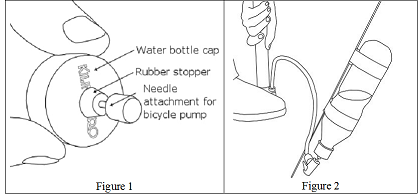
\includegraphics[width=10cm]{./img/bottle-rocket-1.png}
%\end{center}	


\subsection{Bottle Rocket}

\subsubsection*{Learning Objectives}
\begin{itemize}
\item{To observe the effect of Newton's Third Law of Motion}
\end{itemize}

\subsubsection*{Background Information}
Newton's Third Law tells us that, for every action, there is an equal and opposite reaction.  This means that if you apply a force to something, it applies an equal force back on you.  Rockets make use of this principle by ejecting gas at high speeds out of one end so that they are forced in the opposite direction.

\subsubsection*{Materials}
Empty 500 mL water bottle, nail, rubber stopper, straight pin, bicycle pump, needle attachment for pump (the type used to fill a football), tape, old pen, rigid straight wire (approx 1 meter), water

\subsubsection*{Preparation Procedure}
\begin{enumerate}
\item{Make a small round hole (between 0.5 and 1.0 cm in diameter) in the lid of the water bottle by heating a nail and using it to put a hole in the lid.}
\item{Cut a round piece of the rubber stopper so that it can be used to stop this hole.}
\item{Pierce the stopper with a straight pin so that you can pass the needle attachment for a bicycle pump through the stopper.}
\item{Insert the stopper into the hold in the bottle top. The stopper should form a good seal in this hole, and it should be possible to push the stopper through the hole by exerting force on it.}
\item{Insert the needle attachment through the stopper so that you can increase the pressure inside of the bottle.}
\item{Disassemble a pen and take the plastic case.}
\item{Cut the case in half so that you have two hollow cylindrical pieces approximately 3~cm long each.}
\item{Attach them to the side of the bottle using adhesive tape. They should be in a straight line with each other.} 
%!!!
\end{enumerate}

\subsubsection*{Activity Procedure}
\begin{enumerate}
\item{Insert the rigid straight wire into the ground outside.}
\item{Fill approximately half the bottle with water.}
\item{Push the stopper into the inside of the lid.}
\item{Put the needle attachment through the stopper.}
\item{Put the lid on the water bottle and tighten it so that air cannot escape.}
\item{Pass the rigid wire through the pen cylinders and lower the bottle to the ground.}\item{Pump the bicycle pump until the stopper is pushed out completely.}
\end{enumerate}

\subsubsection*{Hazards and Safety}
\begin{itemize}
\item{This is a rocket and will take off quickly and travel far.  Be sure that no one is standing in the way of the rocket, and launch it in a large, open space where no one and nothing can be hit by it.}
\end{itemize}

\subsubsection*{Results and Conclusions}
Once the pressure in the bottle becomes great enough, the stopper will be forced out of the bottle, and the rocket will fly into the air. It should be possible to reach a height of 10 meters or more.  When the stopper leaves the bottle, pressurized air forces water out of the bottom of the bottle at a high speed. Just as with the matchstick rocket, this results in a reaction force forwards on the rocket.
We can also consider this from the perspective of conservation of momentum.


\subsubsection*{Discussion Questions}
\begin{enumerate}
\item{What causes the rocket to launch?}
\item{Explain the two opposing forces present in this experiment.}
\end{enumerate}

\subsubsection*{Notes}
All rockets use this principle; that rapidly expanding gases in one direction causes motion in the opposite direction.  This combines Newton's third law and conservation of momentum.
This activity takes practice. Test this several times before doing it with students.


%\subsection{Matchstick Rocket}
%\begin{itemize}
%\item{Preparation time: 5 minutes}
%\item{Materials: Matches, straight pin, metal foil, scissors, small rock}
%\item{Construction:
%\begin{itemize}
%\item{For this demonstration, I have found that the metal foil from underneath the lid of a Blue Band container works best. If using this foil, make sure you have cleaned off any Blue Band that may have adhered to it. Normal aluminum foil works as well.}
%\item{Different brands of matches work better or worse. Best results have been found with Lucky brand matches, although others have also worked well (the current record for Kasuku matches is 3m). You should attempt this demonstration once or twice yourself with a certain type of matches before doing it in from of the class.}
%\item{Cut out a rectangular piece of foil approximately 2cm x 4cm. Place the straight pin along the length of the match, with the point of the pin touching the match head (see figure 1). Wrap the foil tightly around the match and pin, with about half of the foil extending past the tip of the match (see figure 2). Fold the extra foil securely down over the tip of the match (see figure 3). Remove the straight pin. You have now finished constructing a matchstick rocket.}
%\end{itemize}
%} % Construction
%\item{Procedure: Prop the matchstick rocket on two small, smooth rocks so that it is at approximately a 45° angle. Light another match and hold it underneath for several seconds (see figure 4). The heat will cause the matchstick rocket to ignite. It should fire for a distance of between one and five meters.\\
%Once you have practiced on several matchstick rockets, you should be able to make several of them per minute. It is therefore easy and worthwhile to bring several of them to class, so that you can repeat the demonstration several times. This also gives you an opportunity to invite several students to launch a rocket themselves. If time permits, have a contest to see who can get the best distance on a rocket.}
%\item{Theory: When the matchstick rocket ignites, rapidly expanding hot gases are produced. These are only able to escape by following the pathway left behind by the straight pin. The hot gases are forced backwards from the rocket at a high speed. Newton’s Third Law of Motion tells us that for every force there is an equal and opposite counter-force. Because the hot gases are being forced backwards, there must be a counter-force pushing the rocket forwards.\\
%Alternately, we can consider Conservation of Momentum. Initially, the matchstick rocket is at rest. Once it ignites, hot gases develop a backwards velocity. Because momentum must be conserved, some other part of the system must develop a forward velocity. Thus, the rocket will fly forwards.}
%\end{itemize}
%
%\begin{center}
%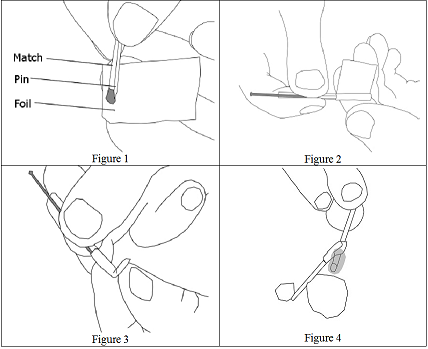
\includegraphics[width=10cm]{./img/matchstick-rocket-1.png}
%\end{center}



\subsection{Matchstick Rocket}

\subsubsection*{Learning Objectives}
\begin{itemize}
\item{To explain the mode of action of a rocket} 
\item{To apply Newton's Third Law to the motion of a rocket} 
\item{To understand the application of Newton's Third Law to propulsion} 
\end{itemize}

\subsubsection*{Background Information}
The motion of a rocket is due to the simple principle of reaction.  Newton's third law explains that a force in one direction will be opposed by a force in the opposite direction.  In other words, if an object pushes backwards against an obstacle, the obstacle will push forward on the object.  When a match burns, the gases that are produced are very hot and expand rapidly. In order for the match to continue burning, the match pushes the gases backwards, and the gases need to escape.

\subsubsection*{Materials}
Matches, aluminium foil, pin or syringe needle

\subsubsection*{Hazards and Safety}
\begin{itemize}
\item{When the rocket ignites, some foil and hot air may be expelled, so no one should be very close. When igniting it yourself, keep your face away from the rocket.} 
\end{itemize}

\subsubsection*{Preparation Procedure}
If you are using a syringe needle instead of a pin, break the needle near the plastic base so that your needle is only the metal part.

\subsubsection*{Activity Procedure}
\begin{enumerate}
\item{Cut or rip a small piece of foil, about 2 cm x 3 cm. Make sure it is flat and does not contain any holes.} 
\item{Hold the pin next to a match so that the tip of the pin touches the head of the match.} 
\item{Hold the pin and match tightly together and wrap the foil around the head of the match (with the pin) so that about 1 cm of foil covers the match and pin, and about 1 cm extends beyond the tip of the match and pin. Wrap the foil tightly so that no openings can be seen around the shaft of the match and pin.} 
\item{Fold the extra foil down over the match head tightly so that there are no openings.} 
\item{Remove the pin by sliding it out of the bottom of the foil, leaving a thin tunnel.} 
\item{Support the match rocket at a 45-degree angle on a stone or other object. Make sure that no one is standing in front of the rocket.} 
\item{Light another match and hold it under the foil of the rocket to ignite the first match. It may take a few seconds to work.} 
\item{Repeat all steps until you have a good rocket.} 
\end{enumerate}

\subsubsection*{Results and Conclusions}
The matchstick rocket moves forward quickly when the match-head ignites inside the foil.  The match moves forward because the gases are moving backward; a force in one direction must be balanced by an equal force in the opposite direction.  

\subsubsection*{Clean Up Procedure}
Return the supplies to their proper places.

\subsubsection*{Discussion Questions}
\begin{enumerate}
\item{What causes the rocket to move forward?}
\item{Where do the gases from combustion of the match go when the rocket ignites?}
\item{What would happen if the exhaust hole left by the pin was facing another direction?}
\item{What would happen if you increase the amount of gas escaping from the match?}
\item{What would happen if you increase the weight of the match?}
\end{enumerate}

\subsubsection*{Notes}
As a match ignites, the gases quickly expand. By removing the pin from the foil over the match head, you leave a small path for the gases to expand: they cannot go any other direction but backward. Newton's Third Law tells us that ``For every action (or force) there is an equal and opposite reaction." The action in this case is the rapid movement of gases backward. The reaction produced is the movement of the matchstick forward.